\documentclass[a4paper, top=10mm]{article}
%for writing from the top
\usepackage{fullpage}
%for math
\usepackage{amsmath}
\usepackage{mathrsfs}
\usepackage{amsthm}
%for images
\usepackage{graphicx}
\usepackage{wrapfig}
%for link
\usepackage{url}
%for color
\usepackage{xcolor}
%for title
\title{\textbf{\huge{Santa's Reindeer}}}
\author{Enigma n\textsuperscript{o}6}
\date{14\textsuperscript{th} December 2023}

\newtheorem*{hint}{Hint}

\addtolength{\voffset}{-2cm}
\addtolength{\textheight}{5cm}


\begin{document}
	\maketitle
	
	\begin{wrapfigure}[18]{r}{0.50\textwidth}
		\vspace{-2cm}
		\hspace{-0.5cm}
		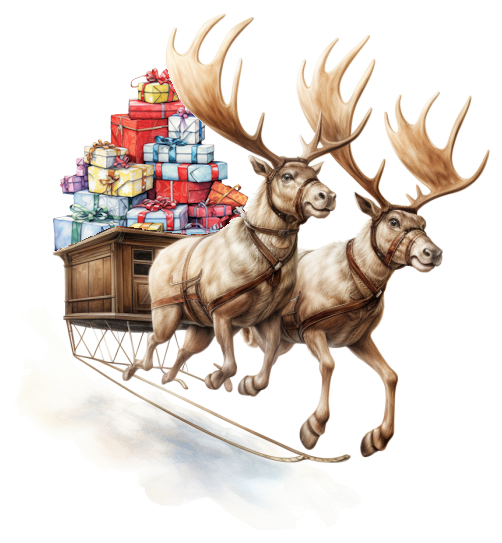
\includegraphics[height=300pt]{06sleigh_with_presents.png}
	\end{wrapfigure}
	
	Santa Claus enters your street.
	He left his sleigh with the reindeer while delivering presents.
	
	You would like to know how many stops Santa Claus has done so far.
	Given that it's early night, you assume it may not be more than $127$ (included).
	
	The reindeer are very smart, they can understand some of your questions.
	The questions must be of the form “Have you done more, less, or exactly $N$ stops so far”?
	And the only three answers that the reindeer can bellow are:
	\begin{itemize}
		\item “Mooooooore”
		\item “Leeeeeeess”
		\item “Exaaaaaact”
	\end{itemize}
	You must be fast: when Santa Claus comes back, you won't be able to ask any other question.
	You figured that you can only ask $7$ questions before Santa Claus comes back.
	
	\begin{center}
		
\includegraphics[height=150pt]{06QR.png}
		
		\url{https://mics-lab.github.io/Enigmas-Xmas2023/enigma6/}
	\end{center}
	
	The QR code / link above will lead you to a simulation of the reindeer.
	
	\textbf{You will be able to ask $7$ questions.}
	
	\textit{A validation code will be given to you if and only if you get “exact” within the 7 allowed questions.}
	
\end{document}